
\section{EXAMPLES OF CIRCUITS}


\subsection{DEFINITION}

A Circuit ( in a digital logic ) is a system made up of logic gates that processes input signals ( usually represented as 0s and 1s ) to produce an output based on a defined rule or function.
\\
Basically, circuits are designed to perform useful functions.. They take inputs (e.g x,y, and z) and produce an output using Boolean logic. The behavior of a circuit can be described using a Boolean expression.

\subsection{Examples}

The following are some examples of circuits and their solutions.


\subsection{EXAMPLE 1}
 A committee of three individuals decides on issues for an organization. Each individual vote yes or no for each proposal that arises. A proposal is passed if it receives at least two yes votes. Design a circuit that determines whether a proposal passes.

\textbf{Solution:}
Let $x=1$ if the first individual votes yes and $x=0$ if this individual votes no; let $y=1$ if the second individual votes yes and $y=0$ if this individual votes no; let $z=1$ if the third individual votes yes and $z=0$ if this individual votes no. Then a circuit must be designed that produces the output 1 when two or more of $x,y,z$ are 1. One Boolean expression for this is
\[
xy+xz+yz.
\]
\begin{figure}[H]
    \centering
    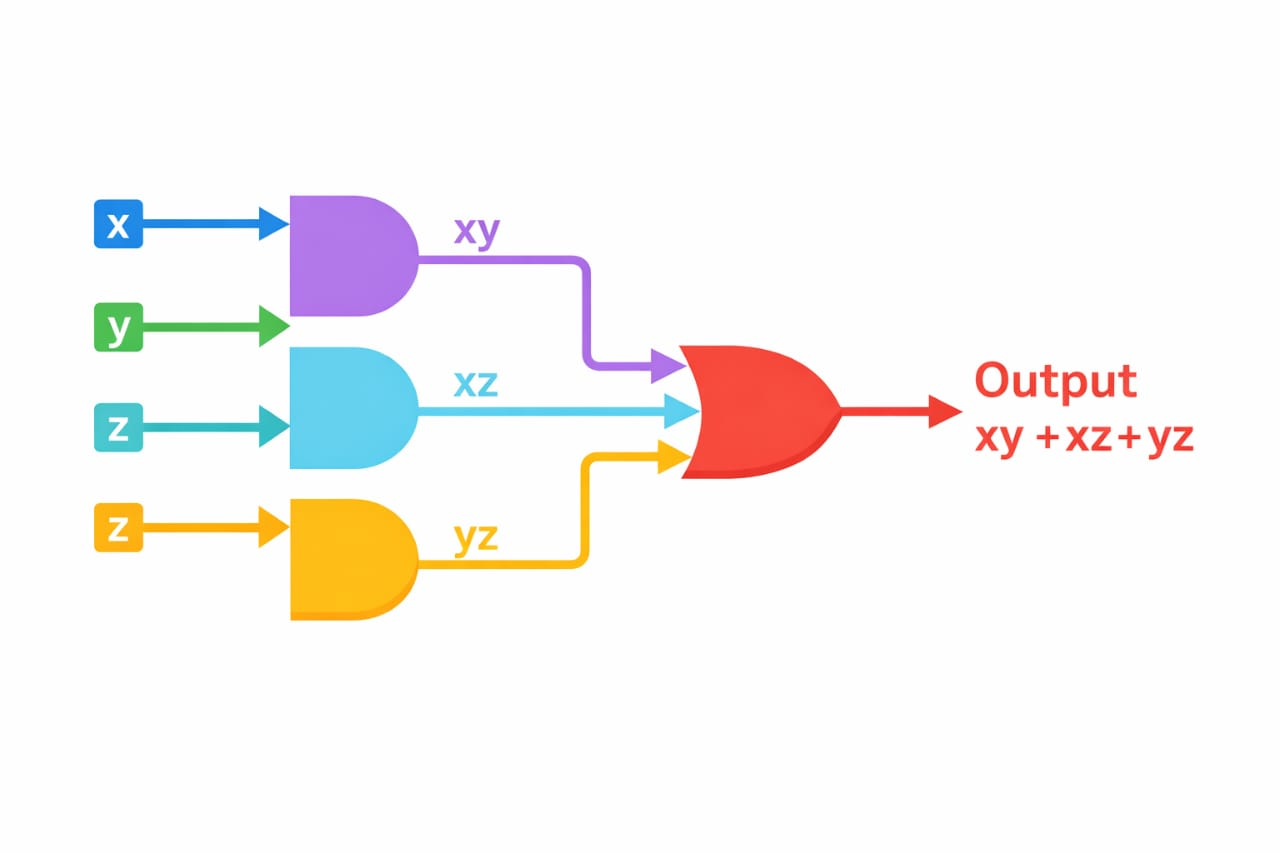
\includegraphics[width=0.75\linewidth]{WhatsApp Image 2026-04-13 at 20.37.12.jpeg}
    \caption{Figure 5: A circuit for Majority Voting}
    \label{fig:placeholder}
\end{figure}

\subsection{EXAMPLE 2}

Sometimes light fixtures are controlled by more than one switch. Circuits need to be designed so that flipping any one of the switches for the fixture turns the light on when it is off and turns the light off when it is on. Design circuits that accomplish this when there are two switches and when there are three switches.

   \textbf{Solution:}
 We begin by designing the circuit that controls the light fixture when two different switches are used. Let $x=1$ when the first switch is closed and $x=0$ when it is open and let $y=1$ when the second switch is closed and $y=0$ when it is open. Let $F(x,y)=1$ when the light is on and $F(x,y)=0$ when it is off. We can arbitrarily decide that the light will be on when both switches are closed, so that $F(1,1)=1$. This determines the remaining values:



\begin{figure}[H]
    \centering
    
\includegraphics[width=0.75\linewidth]{image.png}
    \caption{Enter Caption}
    \label{fig:placeholder}
\end{figure}


\section*{{ADDERS}}

An adder is a digital logic circuit in electronices that implement the addition of numbers.
Half adder: is a combinational circuit that performs the addition of two bits, this circuit needs two binary inputs and two binary outputs.
Adding two single-bit binary values, X and Y produces a sum S bit and a carryout C-out bit.





\textbf{TABLE 3: Input and Output for the Half Adder}

\[
\begin{array}{|c|c||c|c|}
\hline
\multicolumn{2}{|c||}{\textbf{Input}} & \multicolumn{2}{c|}{\textbf{Output}} \\
\hline
x & y & s & c \\
\hline
1 & 1 & 0 & 1 \\
\hline
1 & 0 & 1 & 0 \\
\hline
0 & 1 & 1 & 0 \\
\hline
0 & 0 & 0 & 0 \\
\hline
\end{array}
\]

\vspace{0.5cm}



\begin{figure}[H]
    \centering
    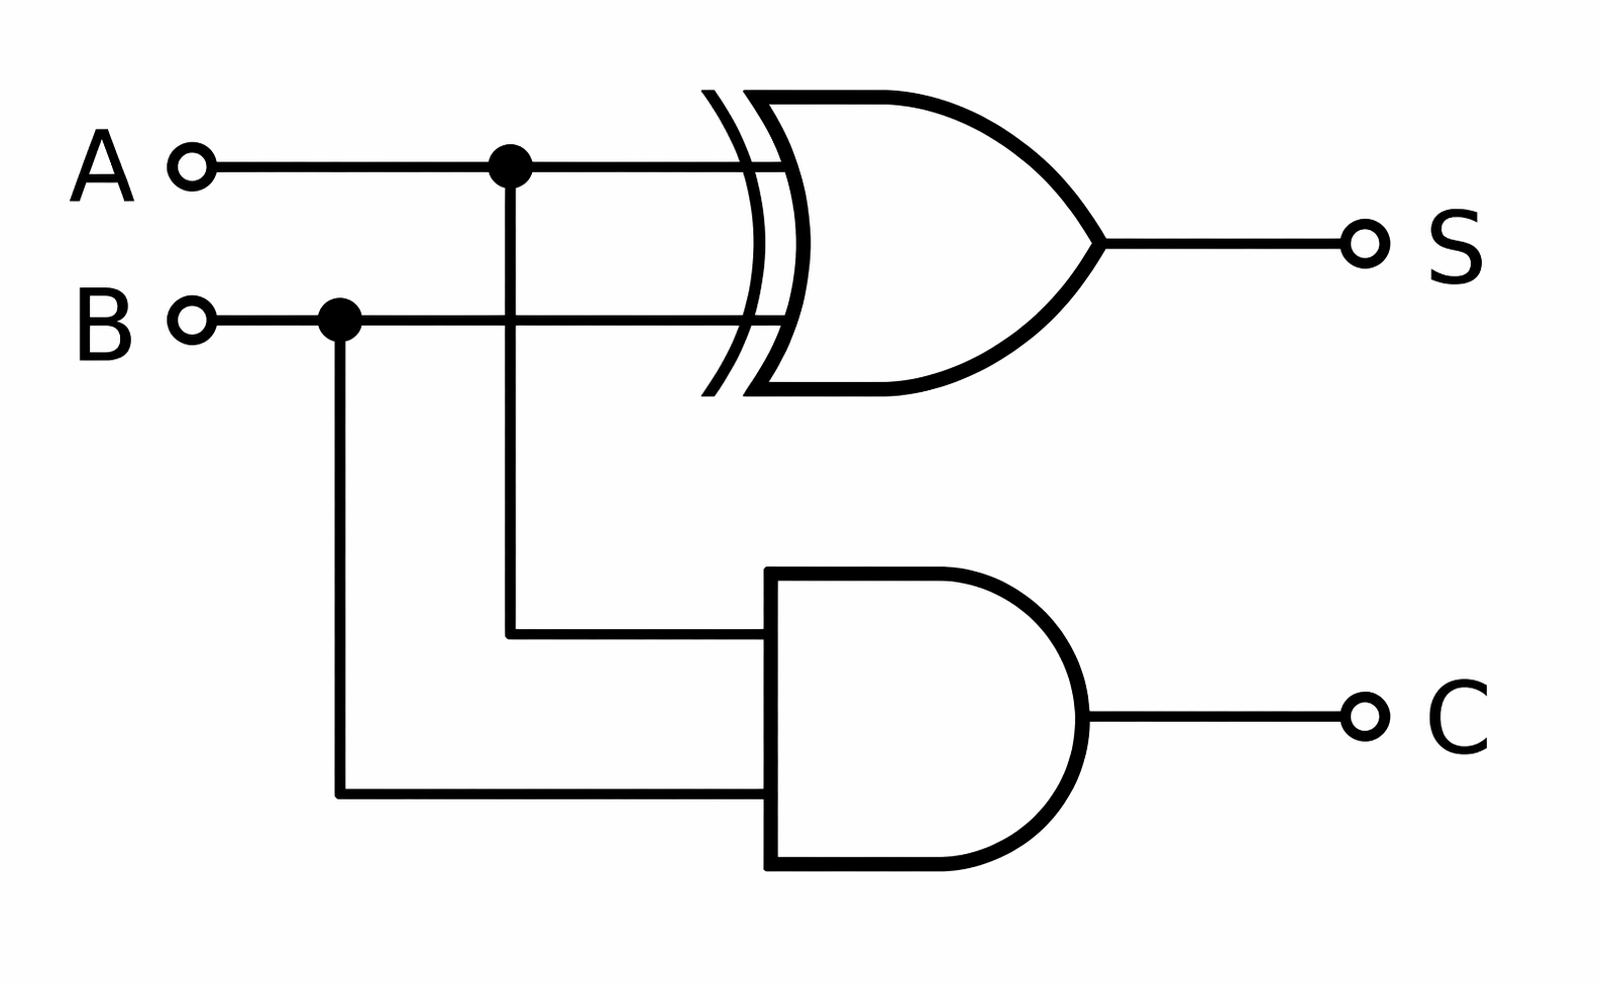
\includegraphics[width=0.6\textwidth]{images/image.png}
    \caption{FIGURE 7: The Half Adder}
    \label{fig:half_adder}
\end{figure}


\section* {Full Adder}

A full adder is a combinational circuit that performs the addition of three bits (two significant bits and a previous carry).
.it consists of three outputs and two outputs, where two inputs are the bits to be added , the third input represent the carry from the previous position.
. Adding two single-bit binary values Xand Y with a carry input bit C-in produces a sum bit Sand a carry out C-out bit.

 The Boolean expressions for the full adder are
\[
s = xyc_i + x\bar{y}\bar{c_i} + \bar{x}y\bar{c_i} + \bar{x}\bar{y}c_i
\]
and
\[
c_{i+1} = xyc_i + xy\bar{c_i} + x\bar{y}c_i + \bar{x}yc_i.
\]
These expressions account for all possible combinations of the three inputs and ensure that the correct sum and carry values are produced. The full adder is more powerful than the half adder because it allows the inclusion of carry propagation, which is essential for performing addition on numbers with more than one bit.

\begin{center}
\textbf{{TABLE 4}}\\[0.2cm]
\textbf{Input and Output for the Full Adder}
\[
\begin{array}{|c|c|c||c|c|}
\hline
\multicolumn{3}{|c||}{\textbf{Input}} & \multicolumn{2}{c|}{\textbf{Output}}\\
\hline
x & y & c_i & s & c_{i+1} \\
\hline
0 & 0 & 0 & 0 & 0 \\
\hline
0 & 0 & 1 & 1 & 0 \\
\hline
0 & 1 & 0 & 1 & 0 \\
\hline
0 & 1 & 1 & 0 & 1 \\
\hline
1 & 0 & 0 & 1 & 0 \\
\hline
1 & 0 & 1 & 0 & 1 \\
\hline
1 & 1 & 0 & 0 & 1 \\
\hline
1 & 1 & 1 & 1 & 1 \\
\hline
\end{array}
\]
\end{center}


\begin{figure}[H]
    \centering
    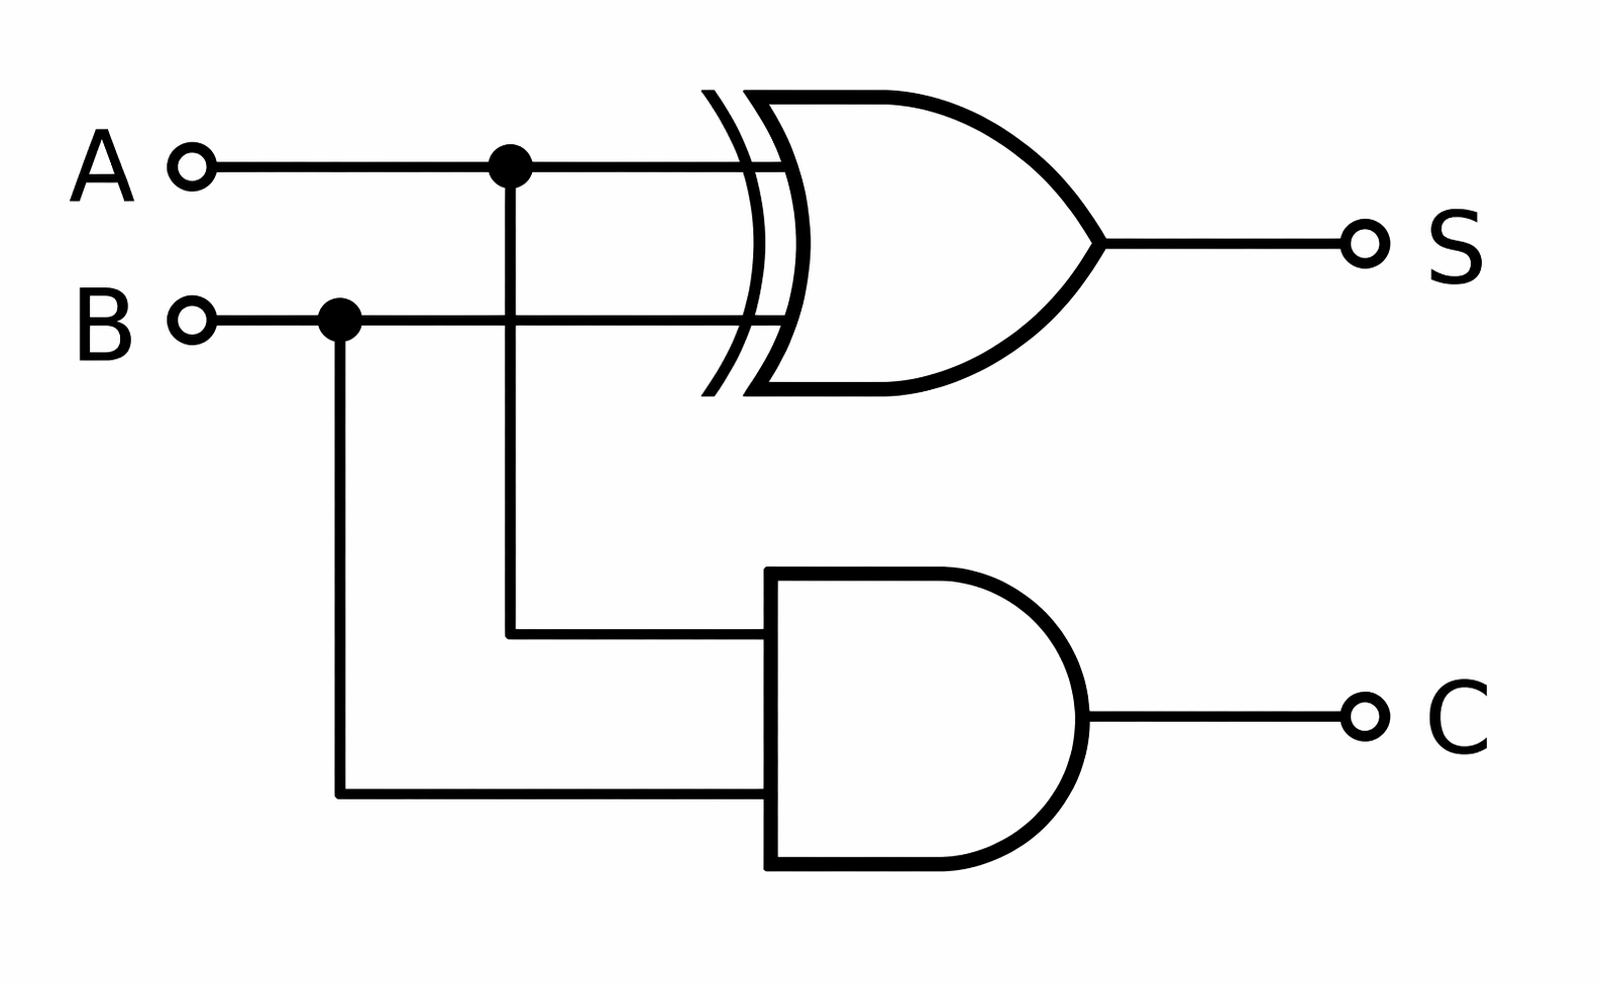
\includegraphics[width=0.7\textwidth]{images/image.png}
    \caption{FIGURE 8: The Full Adder}
    \label{fig:full_adder}
\end{figure}


\section{EXCERCISES}

\textbf{1.} Design a circuit that implements majority voting for five individuals.

\vspace{0.3cm}

\textbf{2.} Design a circuit for a light fixture controlled by four switches, where flipping one of the switches turns the light on when it is off and turns it off when it is on.

\vspace{0.3cm}

\textbf{3.} Show how the sum of two five-bit integers can be found using full and half adders.

\vspace{0.3cm}





\textbf{4.} Construct a circuit that compares the two-bit integers $(x_1x_0)_2$ and $(y_1y_0)_2$, returning an output of 1 when the first of these numbers is larger and an output of 0 otherwise.

\vspace{0.3cm}


